% List all the elements that are directly related to or to the benefit
% of the player.

% Devise two sets of names for player elements. One set is a generic name
% (or code) and the other is its game name. 

% Describe the terminology that you use to describe the player’s
% properties.
\subsection{Elementer}
Dette avsnittet forteller om de forskjellige spillelementene som finnes
i Garbage Alert.
\subsubsection{Ressurser}
Ressurser er et viktig element i Garbage Alert. Ressursene er det som
gjør at spillere kan utvikle basen sin, bygge forsvar og utvikle angrep.
Valget av ressurser er basert på Mohs hardhetsskala av mineraler \cite{mohs}. Mohs hardhetskala er en liste over mineraler i rekkefølge etter absolutt hardhet, laget av geologen Friedrich Mohs. Hvert mineral skal kunne skrape mineralet som står foran på listen. Ressursene i Garbage Alert er ikke helt korrekte i forhold til Mohs hardhetsskala, men basert på denne. Idèen er at hver de seks ressursene i spillet følger samme regel, nemlig at den ene ressursen er hardere enn den andre og har mulighet til å ødelegge den. 
De forskjellige typene utvinnbare ressurser er:
\begin{description}
	\item \textbf{Papp}\\ Denne ressursen kan utvinnest uten å måtte
oppgradere miljøstasjonen. Dette er den enkleste ressursen å få fatt i,
men skaper kun relativt svake angrep/forsvar.
	\item \textbf{Plast}\\ Denne ressursen kan man utvinne etter å ha
oppgradert hovedbasen èn gang.
	\item \textbf{Tre}\\ Tre kan utvinnest dersom hovedbasen har blitt
oppgradert til dette. Tre er på samme oppgraderingsnivå som plast, med andre ord må
spilleren velge mellom desse to i begynnelsen. Tre er derimot hardere enn plast i dette spillet.
	\item \textbf{Jern}\\ Jern er mulig å utvinne dersom spilleren først
oppgraderer til tre.
	\item \textbf{Stål}\\ Stål bygger på at spilleren først har
oppgradert til plast.
	\item \textbf{Titan}\\ Titan er den siste ressursen som er mulig å
utvinne. For å kunne utvinne titan må spilleren først ha skaffet seg
alle utvinningsutvidelsene til hovedbasen.
\end{description}


Det er også mulig å skade forsvar/våpen som er bygget av en bedre ressurs enn våpenet. Dette er implementert slik at ingen våpen/forsvar blir uovervinnelige. Figur \ref{fig:ressursoppgraderinger} framstiller hvilke utvidelser man må ha for å kunne oppgradere til neste nivå. Allerede helt fra starten av spillet må man velge om man først vil oppgradere til tre, eller til plast.

	\begin{figure} [H]
				\begin{center}
					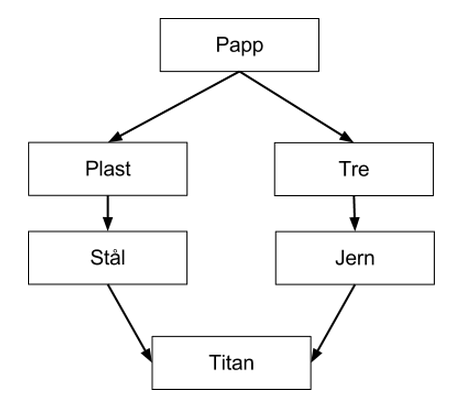
\includegraphics[scale=0.5]{images/oppgraderingstre}
				\end{center}
			\caption{Ressursoppgraderinger}
			\label{fig:ressursoppgraderinger}
	\end{figure}

\subsubsection{Ressursutvinning}
En spiller skaffer seg ressurser ved å gjenvinne søppel som ligger
spredt rundt på øya. Dette blir gjort ved hjelp av gjenvinningsstajonen
som hver spiller starter med.
\subsubsection{Gjenvinningsstasjonen}
Gjenvinningstasjonen er det mest sentrale spillelementet i Garbage
Alert. Denne kan bli sett på som hovedbasen i spillet.
Gjenvinngsstasjonen kan oppgraderes på tre måter for å forbedre effektiviteten:\\
\begin{description}
	\item \textbf{Effektivitet}\\Hvor fort den prosesseserer en enhet søppel (dette starter seint og går raskere for hver oppgradering).
	\item \textbf{Volum/Utvinningsgrad}\\Hvor mye av søppelet som faktisk blir gjennvunnet. “Restavfallet” vil på magisk vis bli borte. Figur \ref{fig:effektivitet} under viser de mulige oppgraderingene for effektivitet og volum/utvinningsgrad. For å oppgradere til nivå 2 må man tidligere ha oppgradert til nivå 1.
	\item \textbf{Buffer}\\Stasjonen kan få en buffer hvor spilleren kan samle opp søppel, som automatiserer gjenvinningsprosessen til en viss grad.
	\item \textbf{Ressurser}\\For å kunne utvinne nye typer ressurser må
		spilleren oppgradere gjenvinningsstasjonen. Her får spilleren valget
		mellom to ulike veier som vil avgjøre hvilke ressurser spillern får
		tilgang til.
\end{description}



		\begin{figure} [H]
				\begin{center}
					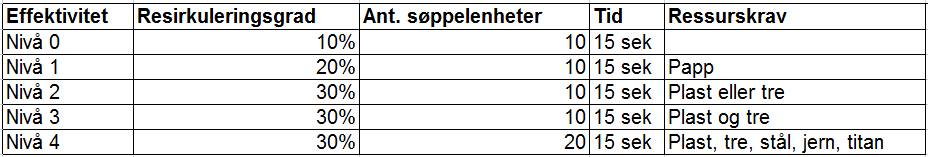
\includegraphics[scale=0.5]{images/effektivitet}
				\end{center}
			\caption{De ulike oppgraderingingene for effektivitet. Ved 10\% resirkuleringsgrad og 10 søppelenheter for man 1 enhet med ressurser per ressursoppgradering man har}
			\label{fig:effektivitet}
		\end{figure}



\subsubsection{Forsvar}
Spillere kan bygge forsvar rundt øya si. Dette forsvaret vil forhindre
motspillere å angripe gjenvinningsstasjonen. Det vil finnes ulike typer
forsvarsmurer, som er kraftige/svake mot ulike typer angrep.
\subsubsection{Angrep}
En spiller får utdelt tre angrepsplattformer. På desse tre platformene
kan spilleren velge hvilke angrep han vil utvikle, basert på hvilke
tilgjengelige ressurser han har.
\subsubsection{Oppgraderinger}
Spilleren har mulighet til å oppgradere både gjenvinningsstasjonen,
våpen og forsvar. Hver type våpen og forsvar har tre nivå, der øking i
nivå vil gi hhv. kraftigere angrep og sterkere forsvar. De tre
våpenplassene på øya kan ha inneholde ulike våpen som kan oppgraderes
hver for seg.
Eksempel på forsvarsoppgradering:\\
Tremur (nivå 1) -> Tremur (nivå 2) -> Tremur (nivå 3).
\begin{quote}
Bør restruktureres!!\\
Spilleren kan utvinne ressurser ved å "dra" søppelenheter fra
forskjellige plasser på øya inn til gjennvinningsstasjonen. Hvilke
ressurser, og mengden av hver ressurs, som spilleren får ut fra en
enkelt søppelenhet er avhengig av nivået på gjennvinningsstasjonen og
hvilke typer oppgraderinger som er gjort. Spilleren kan også bruke sine
våpen til å bli kvitt søppelenheter. Her vil ubehandlede søppelenheter
kunne skytes på motstandere. Effekten av angrepet avhenger av spillerens
våpen, oppgraderingsnivå på våpenet og motstanderens forsvar. For å
beskytte seg mot angrep kan spilleren bygge mur rundt sin øy. Hvilke
våpen og forsvarsmurer som spilleren kan bygge er avhengig av hvilke
ressurser gjenvinningsstasjonen er i stand til å utvinne. Dette betyr at
valg av typer oppgradering for gjenvinningsstasjonen vil være avgjørende
for utviklingen av spillet.\\
\end{quote}
